\documentclass{beamer}

\usepackage{amsmath}
\usepackage{textcomp}
\usepackage{listings}
\usepackage{lmodern}
\usepackage{hyperref}
\usepackage[T1]{fontenc}
\usepackage{tikz}
\usepackage{anyfontsize}

\usepackage{makecell, tabularx}
\newcolumntype{M}{>{\raggedright\arraybackslash}m}
\renewcommand\tabularxcolumn[1]{M{#1}}
\renewcommand\arraystretch{1.2}
\usetikzlibrary{shapes,shapes.geometric,arrows,fit,calc,positioning,automata,}
\usepackage{pgf-pie}

\usepackage[disable]{todonotes}

% Required for biblatex, but also adds functionality for quotation
\usepackage{csquotes}

% Jason's bibliography format
% % Credit to Gabriel Devenyi for this bibliography cfg:
% % github.com/gdevenyi/mcmaster.latex
% \usepackage[
%   style=numeric-comp,
%   backend=biber,
%   sorting=none,
%   backref=true,
%   maxnames=99,
%   alldates=iso,
%   seconds=true
% ]{biblatex} % bibliography
% \addbibresource{references.bib}
\usepackage[round]{natbib}
\bibliographystyle{plainnat}
\setcitestyle{yysep={;}}
\defcitealias{ISTQB}{Hamburg and Mogyorodi}
\newcommand{\citetISTQB}{\citetalias{ISTQB} (\citeyear{ISTQB})}
\newcommand{\citepISTQB}{\citepalias[\citeyear{ISTQB}]{ISTQB}}
\newcommand{\citealpISTQB}{\citetalias{ISTQB}, \citeyear{ISTQB}}

\lstset{
    language=[latex]tex,
    breaklines=true}

\usetheme{Madrid}

\setbeamertemplate{caption}{\centering\insertcaption\par}

% Change block width
\addtobeamertemplate{block begin}{%
    \centering\large%
    \setlength{\textwidth}{0.9\textwidth}
}{}

% From https://tex.stackexchange.com/a/489625/192195
\BeforeBeginEnvironment{block}{\begin{adjustbox}{minipage={\linewidth}, center}}
    \AfterEndEnvironment{block}{\end{adjustbox}}

\usepackage{adjustbox}

\def\checkmark{\tikz\fill[scale=0.4](0,.35) -- (.25,0) -- (1,.7) -- (.25,.15) -- cycle;} 

% Extra functionality for command parsing
\usepackage{xparse}

\newif\ifnotpaper

%------------------------------------------------------------------------------
% Reused in seminar slides
%------------------------------------------------------------------------------

\def\rqatext{What testing approaches do the literature describe?}
\def\rqbtext{Are these descriptions consistent?}
\def\rqctext{Can we systematically resolve any of these inconsistencies?}

\def\expBasedCatMain{\citeauthor{IEEE2022} categorize experience-based testing
    as both a test design technique and a test practice on the same
    page---twice \citeyearpar[Fig.~2, p.~34]{IEEE2022}!}

\NewDocumentCommand{\perfAsFamily}{s}{%
    \IfBooleanTF#1{\citealp}{\citep}[p.~1187]{Moghadam2019}\footnote{
        The original source describes ``performance testing \dots\ as a family
        of performance-related testing techniques'', but it makes more sense to
        consider ``performance-related testing'' as the ``family'' with
        ``performance testing'' being one of the variabilities
        (see \Cref{perf-test-rec}).}%
}

\def\supersAck{Drs.~Spencer Smith and Jacques Carette have been great
    supervisors in the past and have, both then and now, provided me
    with valuable guidance and feedback}

%------------------------------------------------------------------------------
% Spacing Options
%------------------------------------------------------------------------------

\newcommand{\thesisForceSingleSpacing}{\singlespacing}
\newcommand{\thesisForceDoubleSpacing}{\doublespacing}

%------------------------------------------------------------------------------
% Portable HREFs
%------------------------------------------------------------------------------

% Common variant
\newcommand{\porthref}[2]{\href{#2}{#1}\printOnlyFootnote{\url{#2}}}

% Custom URLs
\newcommand{\porthreft}[3]{\href{#3}{#1}\printOnlyFootnote{\href{#3}{#2}}}
% Inside of some environments, footnote marks aren't registered properly, so we
% need to manually write the "text" part
\newcommand{\porthreftm}[2]{\href{#2}{#1\printOnlyFootnoteMark}}

\newcommand{\formatPaper}[2]{%
    \ifnotpaper
        #1{#2}%
    \else
        \underline{#2}%
    \fi
}

\def\refHelper{\ifnotpaper\else Reference \fi}
\newcommand\multiAuthHelper[1]{\ifnotpaper #1\else #1s\fi}

\newcommand\discrepref[1]{%
    \ifnotpaper
        \labelcref{#1-discrep}%
    \else
        \Cref{#1-discrep}%
    \fi}

\newcommand\ifblind[2]{\IfEndWith*{\jobname}{_blind}{#1}{#2}}

% For `TblrNote`s in the middle of a cell (i.e., with following content)
% From https://topanswers.xyz/tex?q=4758
\ExplSyntaxOn
\NewDocumentCommand \MidTblrNote { m }
{{
            \cs_if_exist:NT \hypersetup { \ExpTblrTemplate { note-border }{ default } }
            {
                \__tblr_hyper_link:nn {#1}
                { \textsuperscript { \UseTblrFont { note-tag } #1 } }
            }
        }}
\ExplSyntaxOff

%------------------------------------------------------------------------------
% Generic "chunks" that get reused
%------------------------------------------------------------------------------

\DeclareDocumentCommand\seeSrcCode{ m m m g }{%
    (see the \href
    {https://github.com/samm82/TestGen-Thesis/blob/#1/scripts/#2.py\#L#3%
        \IfNoValueF {#4} {-L#4}}
    {relevant source code})%
}

\newcommand{\accelTolTest}{astronauts \citep[p.~11]{MorgunEtAl1999}, aviators
    \citep[pp.~27,~42]{HoweAndJohnson1995}, or catalysts
    \citep[p.~1463]{LiuEtAl2023}}

\def\recFigs{\Cref{fig:recoveryGraphs,fig:scalGraphs,fig:perf-graph}}

% Define common footnotes about IEEE testing terms for reuse
\newcommand{\distinctIEEE}[1]{distinct from the notion of ``test #1'' described
    in \Cref{tab:ieeeTestTerms}.}
\newcommand{\notDefDistinctIEEE}[1]{\footnote{Not formally defined, but
        \distinctIEEE{#1}}}
\newcommand{\gerrardDistinctIEEE}[1]{\footnote{``Each type of test addresses a
        different risk area'' \citep[p.~12]{Gerrard2000a}, which is
        \distinctIEEE{#1}}}

% Examples of discrepancies
\NewDocumentCommand\tourDiscrep{s}{%
    \IfBooleanTF#1{t}{T}he structure of tours can be defined as either quite
    general \citep[p.~34]{IEEE2022} or ``organized around a special focus''
    \citepISTQB{}\IfBooleanTF#1{}{.}}
\def\alphaDiscrep{Alpha testing is performed by ``users within the organization
    developing the software'' \citep[p.~17]{IEEE2017}, ``a small, selected
    group of potential users'' \citep[p.~5-8]{SWEBOK2024}, or ``roles outside
    the development organization'' conducted ``in the developer's test
    environment'' \citepISTQB{}.}
\def\loadDiscrep{Load testing is performed with loads ``between anticipated
    conditions of low, typical, and peak usage'' \citep[p.~5]{IEEE2022} or
    loads that are as large as possible \citep[p.~86]{Patton2006}.}

\def\suggSrcs{\href
    {https://github.com/samm82/TestGen-Thesis/issues/14\#issuecomment-1839922715}
    {suggested by Dr.~Carette}}

% Used in parSyns tables
\def\ftrnote{Fault tolerance testing may also be a sub-approach of
    reliability testing \ifnotpaper
        \citetext{\citealp[p.~375]{IEEE2017}; \citealp[p.~7-10]{SWEBOK2024}}%
    \else \cite[p.~375]{IEEE2017}, \cite[p.~7-10]{SWEBOK2024}%
    \fi, which is distinct from robustness testing \citep[p.~53]{Firesmith2015}.}
\def\specfn{See \Cref{spec-func-test}.}
\def\ucstn{See \discrepref{use-case-scenario}.}

%------------------------------------------------------------------------------
% For populating values from files
%------------------------------------------------------------------------------

\ExplSyntaxOn
\ior_new:N \g_hringriin_file_stream

\NewDocumentCommand{\ReadFile}{mm}
{
    \hringriin_read_file:nn { #1 } { #2 }
    \cs_new:Npn #1 ##1
    {
        \str_if_eq:nnTF { ##1 } { * }
        { \seq_count:c { g_hringriin_file_ \cs_to_str:N #1 _seq } }
        { \seq_item:cn { g_hringriin_file_ \cs_to_str:N #1 _seq } { ##1 } }
    }
}

\cs_new_protected:Nn \hringriin_read_file:nn
{
    \ior_open:Nn \g_hringriin_file_stream { #2 }
    \seq_gclear_new:c { g_hringriin_file_ \cs_to_str:N #1 _seq }
    \ior_map_inline:Nn \g_hringriin_file_stream
    {
        \seq_gput_right:cx
        { g_hringriin_file_ \cs_to_str:N #1 _seq }
        { \tl_trim_spaces:n { ##1 } }
    }
    \ior_close:N \g_hringriin_file_stream
}

\ExplSyntaxOff

% Define/read values for Undefined Terms methodology for reuse and calculation!
\ReadFile{\undefTermCounts}{assets/misc/undefTermCounts}

\newcount\TotalBefore
\newcount\UndefBefore
\newcount\TotalAfter
\newcount\UndefAfter

\TotalBefore=\undefTermCounts{1}
\UndefBefore=\undefTermCounts{2}
\TotalAfter=\undefTermCounts{3}
\UndefAfter=\undefTermCounts{4}

\def\approachCount{\undefTermCounts{3}}

\ReadFile{\qualityCounts}{build/qualityCount}
\def\qualityCount{\qualityCounts{1}}

\ReadFile{\parSynCounts}{build/parSynCounts}
\def\parSynCount{\parSynCounts{1}}
\def\selfCycleCount{\parSynCounts{2}}

\ReadFile{\stdSources}{build/stdSources}
\ReadFile{\metaSources}{build/metaSources}
\ReadFile{\textSources}{build/textSources}
\ReadFile{\paperSources}{build/paperSources}

\def\srcCount{\the\numexpr\stdSources{3} + \metaSources{3} + \textSources{3} + \paperSources{3}}

\ReadFile{\stdSmntcDiscBrkdwn}{build/stdSmntcDiscBrkdwn}
\ReadFile{\metaSmntcDiscBrkdwn}{build/metaSmntcDiscBrkdwn}
\ReadFile{\textSmntcDiscBrkdwn}{build/textSmntcDiscBrkdwn}
\ReadFile{\paperSmntcDiscBrkdwn}{build/paperSmntcDiscBrkdwn}
\ReadFile{\totalSmntcDiscBrkdwn}{build/totalSmntcDiscBrkdwn}

\ReadFile{\stdSntxDiscBrkdwn}{build/stdSntxDiscBrkdwn}
\ReadFile{\metaSntxDiscBrkdwn}{build/metaSntxDiscBrkdwn}
\ReadFile{\textSntxDiscBrkdwn}{build/textSntxDiscBrkdwn}
\ReadFile{\paperSntxDiscBrkdwn}{build/paperSntxDiscBrkdwn}
\ReadFile{\totalSntxDiscBrkdwn}{build/totalSntxDiscBrkdwn}

\def\stds{\nameref{stds}}
\def\metas{\nameref{metas}}
\def\texts{\nameref{texts}}
\def\papers{\nameref{papers}}
\def\papersTbl{\hyperref[papers]{Papers and Others}}

\def\srcCat{\hyperref[sources]{Source Tier}}
\def\reduns{\ifnotpaper\nameref{redun}\else Redundancies\footnote{Section omitted for brevity.}\fi}

\def\totalDiscreps{\totalSmntcDiscBrkdwn{13}}

\def\cats{\hyperref[cats]{Categories}}
\def\syns{\hyperref[syns]{Synonyms}}
\def\pars{\hyperref[pars]{Parents}}
\def\defs{\hyperref[defs]{Definitions}}
\def\terms{\hyperref[terms]{Terminology}}
\def\cites{\hyperref[cites]{Citations}}

%------------------------------------------------------------------------------
% TODOs
%------------------------------------------------------------------------------

% Generic Inlined TODOs
\newcommand{\intodo}[1]{\todo[inline]{#1}}

% Unimportant TODOs for "later" (i.e., finishing touches or changes immediately before submission)
\newcommand{\latertodo}[1]{\todo[backgroundcolor=Cyan]{\textit{Later}: #1}}

% "Important" TODOs
\newcommand{\imptodo}[1]{\todo[inline,backgroundcolor=Red]{\textbf{Important}: #1}}

% "Easy" TODOs
\newcommand{\easytodo}[1]{\todo[inline,backgroundcolor=SeaGreen]{\textit{Easy}: #1}}
\newcommand{\eztodo}[1]{\easytodo{#1}}

% "Tedious" TODOs
\newcommand{\tedioustodo}[1]{\todo[inline,backgroundcolor=PineGreen]{\textit{Needs time}: #1}}

% "Question" TODO Notes
\newcounter{todonoteQuestionsCtr}
\newcommand{\questiontodo}[1]{\stepcounter{todonoteQuestionsCtr}\todo[backgroundcolor=Lavender]{\textbf{Q \#\thetodonoteQuestionsCtr{}}: #1}}
\newcommand{\qtodo}[1]{\questiontodo{#1}}

% Specific categories of TODOs
\def\ptq{\todo{Present tense?}}

%------------------------------------------------------------------------------
% Citations
%------------------------------------------------------------------------------

\newcommand{\exhInfCite}{(\citealp[p.~5-5]{SWEBOK2024}; \citealp[p.~4]{IEEE2022};
    \citealp[p.~421]{vanVliet2000}; \citealp[pp.~439, 461]{PetersAndPedrycz2000})}

%------------------------------------------------------------------------------
% Link to Drasil issue
%------------------------------------------------------------------------------

\newcommand{\issueref}[1]{\href{https://github.com/JacquesCarette/Drasil/issues/#1}{\##1}}
\newcommand{\pullref}[1]{\href{https://github.com/JacquesCarette/Drasil/pull/#1}{\##1}}
\newcommand{\thesisissuerefhelper}[1]{\href{https://github.com/samm82/TestGen-Thesis/issues/#1}{\##1}}

\ExplSyntaxOn

% Based on output from ChatGPT
\NewDocumentCommand{\mapthesisissueref}{m}
{
    % Clear temporary sequences to store transformed items
    \seq_clear:N \l_tmpa_seq
    \seq_clear:N \l_tmpb_seq

    \seq_set_split:Nnn \l_tmpa_seq { , } { #1 } % Split the input by commas
    \seq_map_inline:Nn \l_tmpa_seq
    {
        \seq_put_right:Nn \l_tmpb_seq {\thesisissuerefhelper{##1}}
    }
    \seq_use:Nnnn \l_tmpb_seq { ~and~ } { ,~ } { ,~and~ }
}

\ExplSyntaxOff

\newcommand{\thesisissueref}[1]{\todo[backgroundcolor=lightgray]{See \mapthesisissueref{#1}}}

\notpapertrue

\renewcommand\stds{\stdSources{1}}
\renewcommand\metas{\metaSources{1}}
\renewcommand\texts{\textSources{1}}
\renewcommand\papers{\paperSources{1}}

\title[Testing Terminology]{Putting Software Testing Terminology to the Test}
\subtitle{M.A.Sc. Seminar}
\author[Samuel Crawford]{Samuel Crawford, B.Eng.}

% Committee
% \begin{itemize}
%     \item \emph{Supervisor}: Dr.~Jacques Carette
%     \item \emph{Supervisor}: Dr.~Spencer Smith
%     \item Dr.~Ned Nedialkov
%     \item Dr.~Richard Paige
% \end{itemize}

\institute[McMaster University]{McMaster University\\Department of Computing and Software}
\date{Fall 2024}

\AtBeginSection[]
{
  \begin{frame}
    \frametitle{Table of Contents}
    \tableofcontents[currentsection]
  \end{frame}
}

\begin{document}

% From https://tex.stackexchange.com/a/42826/192195
\NewDocumentCommand{\ShowListingForLineNumber}{s O{1.0} m m}{
    \IfBooleanTF{#1}{\vspace{-#2\baselineskip}}{}
    \lstinputlisting[
        style=MyListStyle,
        linerange={#3-#3},
        firstnumber=#3,
    ]{#4}
}

%%%%%%%%%%%%%%%%%%%%%%%%%%%%%%%%%%%%%%%%%%%%%%%%%%%%%%%%%%%%%%%%%%%%%%%%%%%%%%%
%% TITLE PAGE
%%%%%%%%%%%%%%%%%%%%%%%%%%%%%%%%%%%%%%%%%%%%%%%%%%%%%%%%%%%%%%%%%%%%%%%%%%%%%%%
\frame{\titlepage}

%%%%%%%%%%%%%%%%%%%%%%%%%%%%%%%%%%%%%%%%%%%%%%%%%%%%%%%%%%%%%%%%%%%%%%%%%%%%%%%
%% TABLE OF CONTENTS
%%%%%%%%%%%%%%%%%%%%%%%%%%%%%%%%%%%%%%%%%%%%%%%%%%%%%%%%%%%%%%%%%%%%%%%%%%%%%%%

\begin{frame}
    \frametitle{Table of Contents}
    \tableofcontents
\end{frame}

%%%%%%%%%%%%%%%%%%%%%%%%%%%%%%%%%%%%%%%%%%%%%%%%%%%%%%%%%%%%%%%%%%%%%%%%%%%%%%%
%% INTRODUCTION
%%%%%%%%%%%%%%%%%%%%%%%%%%%%%%%%%%%%%%%%%%%%%%%%%%%%%%%%%%%%%%%%%%%%%%%%%%%%%%%
\section{Introduction}

\subsection{The Need for Standardized Terminology}

\begin{frame}
    \frametitle{The Need for Standardized Terminology}
    \begin{itemize}
        \item Engineering is applied science
        \item Scientific fields use precise terminology
        \item Therefore, the same should be true of software engineering!
        \item <2-> Imagine if other fields used unclear, inconsistent, and
              incorrect terminology:
              \begin{itemize}
                  \item Force
                  \item Isotope
                  \item Phalange
              \end{itemize}
    \end{itemize}
    \begin{block}<3->{}{\litStd{}}
        % \vspace{3mm}
        % \hspace\fill{\small--- Dr.~Jacques Carette}
    \end{block}
\end{frame}

\begin{frame}
    \frametitle{Improved Communication}
    \begin{columns}[T]
        \begin{column}{.5\textwidth}
            \begin{center}
                \huge Interorganizational

                \normalsize Schools, companies, etc.

                \vspace{5mm}

                % Based on code frustratingly generated by ChatGPT
                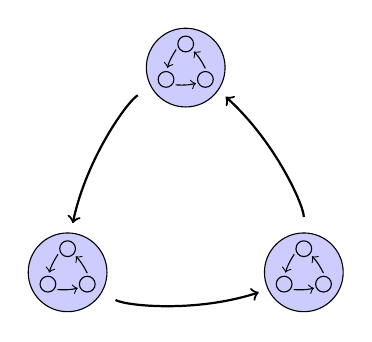
\begin{tikzpicture}

                    % Define coordinates of the triangle's vertices
                    \coordinate (A) at (0, 0);
                    \coordinate (B) at (3, 0);
                    \coordinate (C) at (1.5, 2.6);
                    \coordinate (D) at (1.5, 0.86667);

                    % Draw circles at each vertex without labels
                    \draw[fill=blue!20] (A) circle [radius=0.5];
                    \draw[fill=blue!20] (B) circle [radius=0.5];
                    \draw[fill=blue!20] (C) circle [radius=0.5];

                    % Draw arrows as arcs
                    \draw[->, thick, shorten <= 20pt] (B) arc (0:48:3cm);
                    \draw[->, thick, shorten <= 20pt] (C) arc (120:168:3cm);
                    \draw[->, thick, shorten <= 20pt] (A) arc (240:288:3cm);

                    % Small diagrams inside each circle
                    \only<2->{
                        \foreach \x in {A,B,C} {
                                \begin{scope}[shift={(\x)}, scale=0.2] % Scaling down and shifting to position A
                                    \coordinate (D) at (-1.25, -0.75);
                                    \coordinate (E) at (1.25, -0.75);
                                    \coordinate (F) at (0, 1.5);
                                    \draw[fill=blue!20] (D) circle [radius=0.5];
                                    \draw[fill=blue!20] (E) circle [radius=0.5];
                                    \draw[fill=blue!20] (F) circle [radius=0.5];
                                    \draw[->, shorten <= 4pt] (E) arc (0:45:2.5cm);
                                    \draw[->, shorten <= 4pt] (F) arc (120:165:2.5cm);
                                    \draw[->, shorten <= 4pt] (D) arc (240:285:2.5cm);
                                \end{scope}
                            }
                    }
                \end{tikzpicture}
            \end{center}
        \end{column}
        \begin{column}<2->{.5\textwidth}
            \begin{center}
                \huge Intraorganizational \normalsize
            \end{center}

            \citet[p.~7]{KanerEtAl2011} say ``complete testing'' could require
            the tester to:
            \begin{itemize}
                \item discover ``every bug'',
                \item exhaust the time allocated,
                \item implement every planned test,
                \item \dots{}
            \end{itemize}
        \end{column}
    \end{columns}
\end{frame}

\subsection{The Lack of Standardized Terminology}

\begin{frame}
    \frametitle{The Lack of Standardized Terminology}
    \framesubtitle{``The Problem''}
    \begin{itemize}
        \item \badTaxonomies{}
    \end{itemize}
\end{frame}

\begin{frame}
    \frametitle{Unstandardized Standards}
    \framesubtitle{``The Problem'' (cont.)}
    \begin{itemize}
        \item Tours ``guide[] testers through the paths of an application'' by
              following a structure that is:
              \begin{itemize}
                  \item quite general \citep[p.~34]{IEEE2022}
                  \item<2-> ``organized around a special focus'' \citepISTQB{}
              \end{itemize}
        \item<3-> Load testing is ``conducted to evaluate the behaviour of a
              test item under anticipated conditions of varying load''
              (\citealp[p.~5]{IEEE2022}; \citeyear[p.~253]{IEEE2017}), such as:
              \begin{itemize}
                  \item<3-> loads ``between anticipated conditions of low,
                        typical, and peak usage'' \citeyearpar[p.~5]{IEEE2022}
                  \item<4-> loads that are as large as possible
                        \citep[p.~86]{Patton2006}
              \end{itemize}
    \end{itemize}
\end{frame}

\begin{frame}
    \frametitle{Unstandardized Standards}
    \framesubtitle{``The Problem'' (cont.)}
    \begin{itemize}
        \item Alpha testing is the ``first stage of testing before a product is
              considered ready for commercial or operational use''
              \citep[p.~17]{IEEE2017} performed by:
              \begin{itemize}
                  \item ``users within the organization developing
                        the software'' (p.~17)
                  \item<2-> ``a small, selected group of
                        potential users'' \citep[p.~5-8]{SWEBOK2024}
                  \item<3-> ``roles outside the development organization'' conducted
                        ``in the developer's test environment'' \citepISTQB{}
              \end{itemize}
    \end{itemize}

    \begin{block}<4->{}
        {``Okay testing team, we want to conduct alpha testing on our
            product. What's our timeline? Budget? Sample size?''}
        % \vspace{3mm}
        % \hspace\fill{\small--- Dr.~Jacques Carette}
    \end{block}
\end{frame}

%%%%%%%%%%%%%%%%%%%%%%%%%%%%%%%%%%%%%%%%%%%%%%%%%%%%%%%%%%%%%%%%%%%%%%%%%%%%%%%
%% PROJECT
%%%%%%%%%%%%%%%%%%%%%%%%%%%%%%%%%%%%%%%%%%%%%%%%%%%%%%%%%%%%%%%%%%%%%%%%%%%%%%%

\section{Project}
\subsection{Research Questions}

\def\rqa{\begin{alertblock}{Research Question 1}
        \rqatext{}
    \end{alertblock}
}

\def\rqb{\begin{alertblock}{Research Question 2}
        \rqbtext{}
    \end{alertblock}
}

\def\rqc{\begin{alertblock}{Research Question 3}
        \rqctext{}
    \end{alertblock}
}

\begin{frame}{Research Questions}
    \onslide<1-4>\rqa{}
    \onslide<2-3>\rqb{}
    \onslide<3>\rqc{}
    \onslide<4>
    \vspace{-2.5cm}
    \begin{center}
        \huge{Literature Review Time!}
    \end{center}
\end{frame}

\subsection{Methodology}

\begin{frame}{Methodology: Sources}
    \begin{figure}
        \centering
        \begin{tikzpicture}
            \pie[sum=auto, after number=, text=legend, thick,
                scale=\ifnotpaper0.7\else0.5\fi,
                every label/.style={align=left, scale=0.7}]
            {\stdSources{3}/\stds{},
                \metaSources{3}/\metas{},
                \textSources{3}/\texts{},
                \paperSources{3}/\papers{}}

            \onslide<2>{
                \node[anchor=west, align=left] at (-1.9, 3) {
                    Textbooks trusted at McMaster were our ad hoc starting points\\
                    \quad\quad \citep{Patton2006, PetersAndPedrycz2000, vanVliet2000}
                };
                \draw[->, very thick] (-1.5, 2.85) -- (-1.25, 1.4);
            }

            \onslide<3>{
                \node[anchor=west, align=left] at (2.4, -2) {
                    Includes websites \citetext{\citealp{LambdaTest2024}; \\
                        \quad\quad\citealp{Pandey2023}} and a booklet\\
                    \quad\quad\citep{SPICE2022}};
                \draw[->, very thick] (2.25, -1.5) -- (1.25, -1.1);
            }

        \end{tikzpicture}
        \caption{Summary of how many sources comprise each source category.}
        \label{fig:sourceSummary}
    \end{figure}
\end{frame}

\begin{frame}[t]{Methodology: Categories}
    \vspace{-0.75cm}
    \centering
    \only<1>{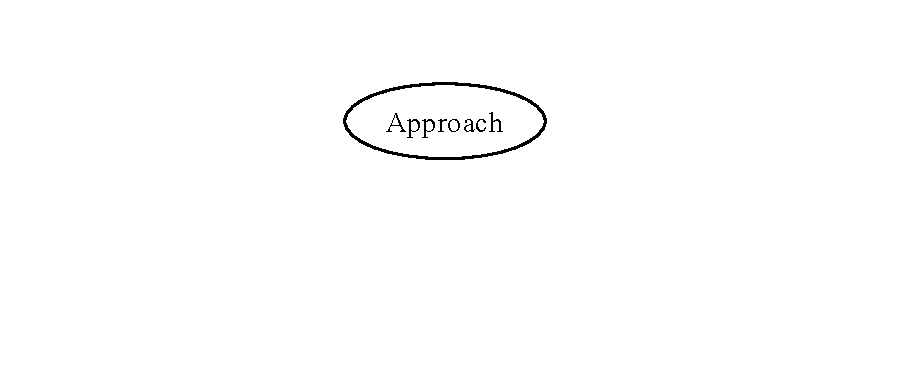
\includegraphics[width=\linewidth]{assets/graphs/manual/catRels1.pdf}}
    \only<2>{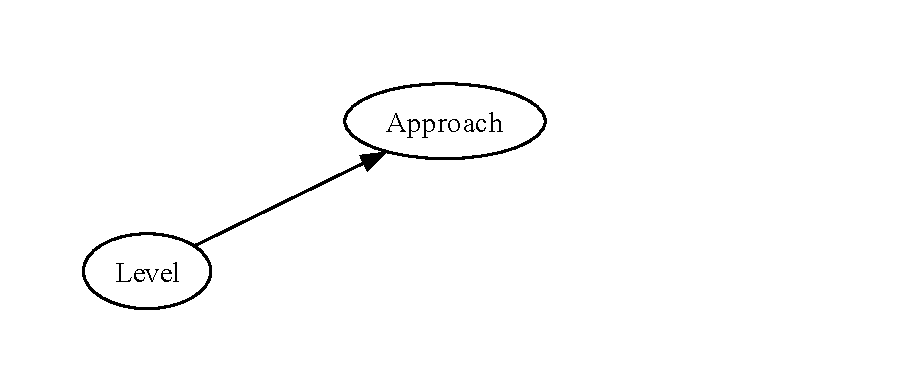
\includegraphics[width=\linewidth]{assets/graphs/manual/catRels2.pdf}}
    \only<3>{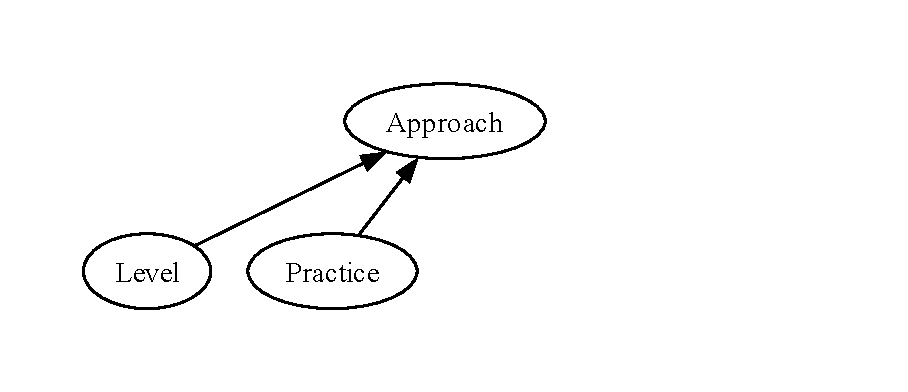
\includegraphics[width=\linewidth]{assets/graphs/manual/catRels3.pdf}}
    \only<4>{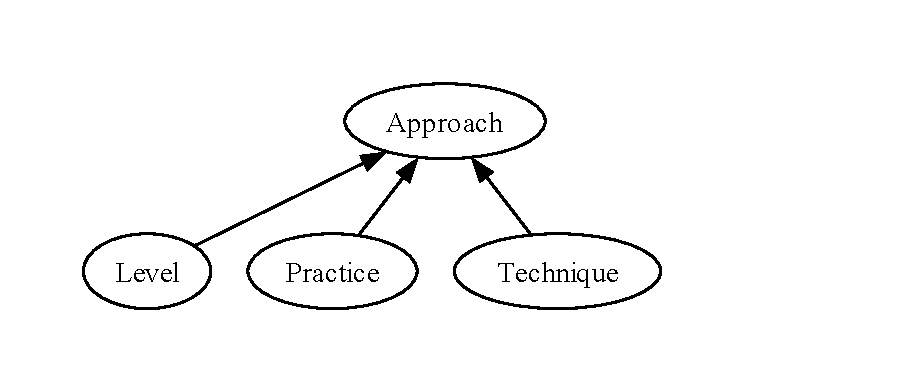
\includegraphics[width=\linewidth]{assets/graphs/manual/catRels4.pdf}}
    \only<5>{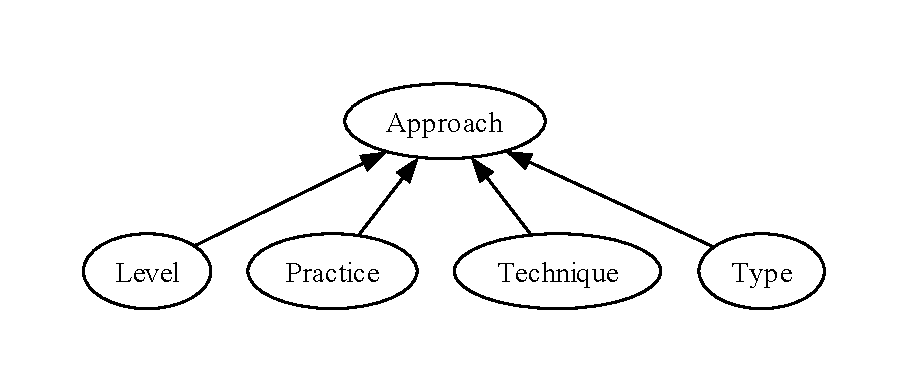
\includegraphics[width=\linewidth]{assets/graphs/manual/catRels5.pdf}}

    \begin{minipage}{0.98\textwidth}
        % For weird spacing issue
        \only<1-3>{\vspace{-0.8cm}}
        \only<4>{\vspace{-0.475cm}}
        \only<5>{\vspace{0.02cm}}
        \only<1>{\textbf{Approach:} a ``high-level test implementation choice''
            \citep[p.~10]{IEEE2022} used to ``pick the particular test case
            values'' \citeyearpar[p.~465]{IEEE2017}}
        \only<2>{\textbf{Level:} a stage of testing with ``particular
            objectives and \dots{} risks'', each performed in sequence
            (\citealp[p.~12]{IEEE2022}; \citeyear[p.~6]{IEEE2021})}
        \only<3>{\textbf{Practice:} a ``conceptual framework that can be applied
            to \dots{} [a] test process to facilitate testing''
            (\citealp[p.~14]{IEEE2022}; \citeyear[p.~471]{IEEE2017})}
        \only<4>{\textbf{Technique:} a ``defined'' and ``systematic''
            \citep[p.~464]{IEEE2017} ``procedure used to create or select a test
            model, identify test coverage items, and derive corresponding test cases''
            \citeyearpar[p.~11]{IEEE2022}}
        \only<5>{\textbf{Type:} ``Testing that is focused on specific quality
            characteristics'' (\citealp[p.~15]{IEEE2022}; \citeyear[p.~7]{IEEE2021};
            \citeyear[p.~473]{IEEE2017})}
    \end{minipage}
\end{frame}

\begin{frame}[t]{Methodology: Graph Notation}
    \vspace{-0.75cm}
    \centering
    \only<1>{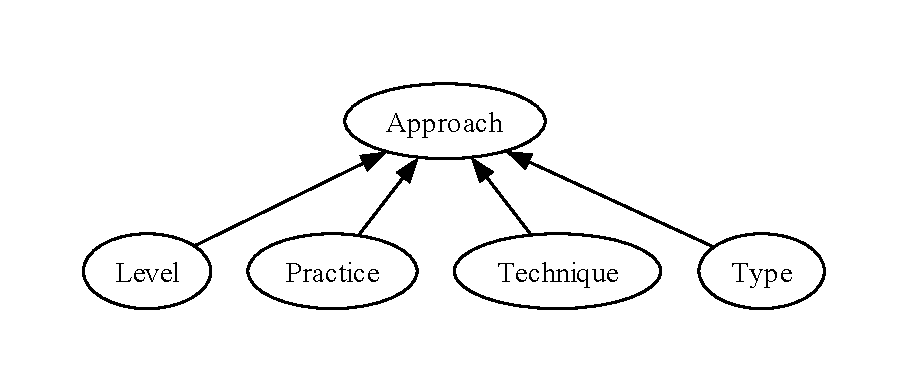
\includegraphics[width=\linewidth]{assets/graphs/manual/catRels5.pdf}}
    \only<2>{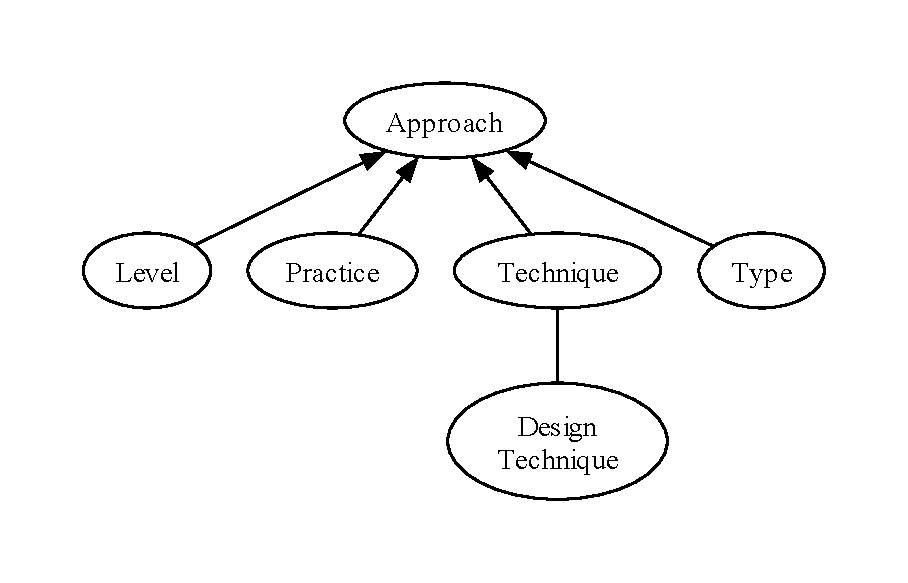
\includegraphics[width=\linewidth]{assets/graphs/manual/catRels6.pdf}}
    \only<3>{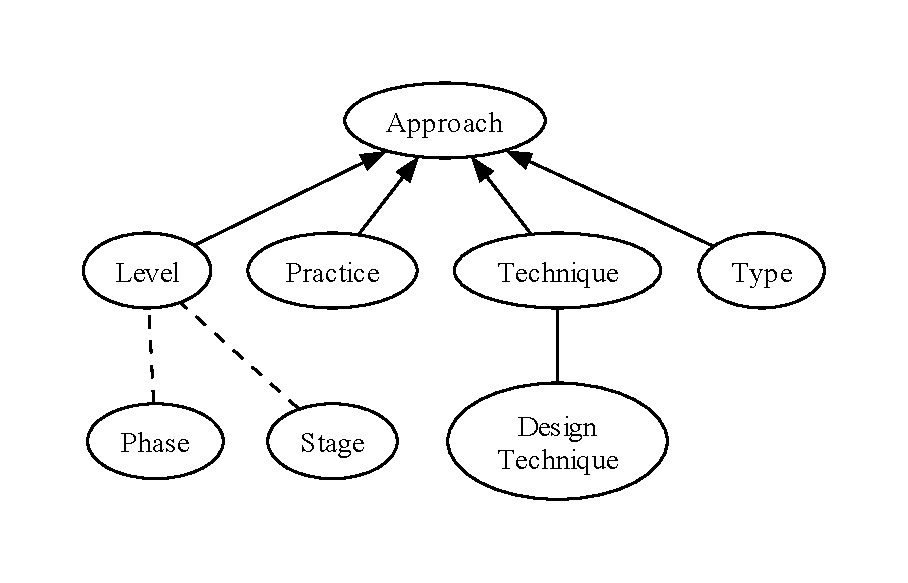
\includegraphics[width=\linewidth]{assets/graphs/manual/catRels7.pdf}}

    \begin{minipage}{0.98\textwidth}
        \centering
        % For spacing issues
        \only<1>{\vspace{1.65cm}}
        \only<2>{\vspace{-2.1cm}}
        \only<3>{\vspace{-1.1cm}}
        \only<1>{Arrows point from a \emph{child} node to a \emph{parent} node.}
        \only<2>{Lines without arrowheads connect \emph{synonyms}.}
        \only<3>{Dashed lines indicate the relationship is \emph{implied}.}
    \end{minipage}
\end{frame}

\begin{frame}{Methodology: Procedure}
    \framesubtitle{Approaches}
    \begin{itemize}
        \item A row is created for each test approach, such as the following which is based on \citep{IEEE2022}
    \end{itemize}
    \begin{center}
        \small
        \begin{tabularx}{\linewidth}{|M{1.1cm}|M{1.4cm}|X|M{1.7cm}|M{1.8cm}|}
            \hline
            \thead{\textbf{Name}} & \thead{\textbf{Category}} & \thead{\textbf{Definition}}                                                                            & \thead{\textbf{Parent(s)}}               & \thead{\textbf{Synonym(s)}}   \\
            \hline
            A/B Testing           & Practice (p.~22)          & Testing ``that allows testers to determine which of two systems or components performs better'' (p.~1) & Statistical Testing (pp.~1,~35), \dots{} & Split-Run Testing (pp.~1,~35) \\
            \hline
        \end{tabularx}
    \end{center}
    \pause
    \begin{itemize}
        \item This information is gathered from sources by looking for
              \begin{itemize}
                  \item Glossaries
                  \item Testing-related terms
                  \item Terms described \emph{by} other approaches
                  \item Terms that \emph{imply} other approaches
              \end{itemize}
    \end{itemize}
\end{frame}

\begin{frame}{Methodology: Procedure}
    \framesubtitle{Other Information}
    \begin{itemize}
        \item It seems that the existence of a software quality implies the
              existence of a test type associated with it \pause
        \item Some test approaches use shared or complicated terminology \pause
        \item For each of these, we record its
              \begin{itemize}
                  \item Name
                  \item Definition
                  \item Precedence for a related test type (only for qualities)
                  \item Synonym(s)
              \end{itemize}
    \end{itemize}
\end{frame}

%   \begin{figure}
%       %   \vspace{-1mm}
%       \includegraphics[width=.8\textwidth]{assets/stable.png}
%       %   \vspace{-3mm}
%       \caption{Contents of \texttt{stable}}
%       \vspace{-1mm}
%   \end{figure}

%   \lstinputlisting[
%       title=An example log,
%       captionpos=b,
%       language={},
%       basicstyle=\tiny, % TODO: reduce font size?
%       breakatwhitespace=true,
%       showstringspaces=false
%   ]{assets/log.txt}

% \onslide<7-|handout:1>\begin{block}{}
%     {"The information you have should be just as useful for generating
%         tests as it should be for manually running them."}
%     \vspace{3mm}
%     \hspace\fill{\small--- Dr.~Jacques Carette}
% \end{block}


%%%%%%%%%%%%%%%%%%%%%%%%%%%%%%%%%%%%%%%%%%%%%%%%%%%%%%%%%%%%%%%%%%%%%%%%%%%%%%%
%% ACKNOWLEDGEMENTS
%%%%%%%%%%%%%%%%%%%%%%%%%%%%%%%%%%%%%%%%%%%%%%%%%%%%%%%%%%%%%%%%%%%%%%%%%%%%%%%

\begin{frame}
    \frametitle{Acknowledgment}

    \begin{itemize}
        \item Dr.~Smith and Dr.~Carette have been great supervisors in the
              past and have, both then and now, provided me with valuable guidance
              and feedback
              \begin{itemize}
                  \item They have helped me refine the scope of this project
                  \item Dr.~Smith first suggested generating test cases back in 2020!
              \end{itemize}
        \item<2-> The format of this presentation was \emph{heavily} based on
              a previous presentation by Jason Balaci, who also provided a
              great thesis template
        \item<3-> The past and current Drasil team have created a truly amazing
              framework!
    \end{itemize}
\end{frame}

%%%%%%%%%%%%%%%%%%%%%%%%%%%%%%%%%%%%%%%%%%%%%%%%%%%%%%%%%%%%%%%%%%%%%%%%%%%%%%%
%% A FINAL THANK YOU
%%%%%%%%%%%%%%%%%%%%%%%%%%%%%%%%%%%%%%%%%%%%%%%%%%%%%%%%%%%%%%%%%%%%%%%%%%%%%%%

\begin{frame}
    \center
    \huge{Thank you!}\\
    \normalsize{Questions?}
\end{frame}

%%%%%%%%%%%%%%%%%%%%%%%%%%%%%%%%%%%%%%%%%%%%%%%%%%%%%%%%%%%%%%%%%%%%%%%%%%%%%%%
%% REFERENCES
%%%%%%%%%%%%%%%%%%%%%%%%%%%%%%%%%%%%%%%%%%%%%%%%%%%%%%%%%%%%%%%%%%%%%%%%%%%%%%%

% From https://tex.stackexchange.com/a/457255/192195
\setbeamertemplate{page number in head/foot}{}

\begin{frame}[allowframebreaks,noframenumbering]
    \frametitle{References}

    \bibliography{references}
\end{frame}

\end{document}
